%%%%%%%%%%%%%%%%%%%%%%%%%%%%%%%%%%%%%%%%%
% Short Sectioned Assignment
% LaTeX Template
% Version 1.0 (5/5/12)
%
% This template has been downloaded from:
% http://www.LaTeXTemplates.com
%
% Original author:
% Frits Wenneker (http://www.howtotex.com)
%
% License:
% CC BY-NC-SA 3.0 (http://creativecommons.org/licenses/by-nc-sa/3.0/)
%
%%%%%%%%%%%%%%%%%%%%%%%%%%%%%%%%%%%%%%%%%

%----------------------------------------------------------------------------------------
%	PACKAGES AND OTHER DOCUMENT CONFIGURATIONS
%----------------------------------------------------------------------------------------

\documentclass[11pt]{article} % A4 paper and 11pt font size

\usepackage[a4paper,margin=1in,footskip=.3in]{geometry}

\linespread{1.0} % Line spacing

\setlength\parindent{0pt} % Removes all indentation from paragraphs - comment this line for an assignment with lots of text
\setlength{\parskip}{6pt}

\usepackage{sectsty} % Allows customizing section commands
\allsectionsfont{\centering \normalfont\scshape} % Make all sections centered, the default font and small caps

\usepackage{fancyhdr} % Custom headers and footers
\pagestyle{fancyplain} % Makes all pages in the document conform to the custom headers and footers
\fancyhead{} % No page header - if you want one, create it in the same way as the footers below
\fancyfoot[L]{} % Empty left footer
\fancyfoot[C]{} % Empty center footer
\fancyfoot[R]{\thepage} % Page numbering for right footer
\renewcommand{\headrulewidth}{0pt} % Remove header underlines
\renewcommand{\footrulewidth}{0pt} % Remove footer underlines
\setlength{\headheight}{13.6pt} % Customize the height of the header

\usepackage[utf8]{inputenc}
\usepackage[T1]{fontenc} % Use 8-bit encoding that has 256 glyphs

\usepackage{fourier} % Use the Adobe Utopia font for the document - comment this line to return to the LaTeX default
\usepackage[english]{babel} % English language/hyphenation

\usepackage{amsmath,amsfonts,amsthm} % Math packages
\theoremstyle{plain}
\newtheorem{theorem}{Theorem}[section]
\newtheorem{corollary}{Corollary}[theorem]
\newtheorem{proposition}[theorem]{Proposition}
\newtheorem{lemma}[theorem]{Lemma}

\theoremstyle{definition}
\newtheorem{definition}{Definition}[section]

\theoremstyle{remark}
\newtheorem*{remark}{Remark}

\numberwithin{equation}{section} % Number equations within sections (i.e. 1.1, 1.2, 2.1, 2.2 instead of 1, 2, 3, 4)
\numberwithin{figure}{section} % Number figures within sections (i.e. 1.1, 1.2, 2.1, 2.2 instead of 1, 2, 3, 4)
\numberwithin{table}{section} % Number tables within sections (i.e. 1.1, 1.2, 2.1, 2.2 instead of 1, 2, 3, 4)

\usepackage{algpseudocode}
\usepackage{algorithm}

\usepackage{listings}

\usepackage{tikz}

\usepackage{natbib}
\bibliographystyle{plainnat}

\usepackage{lipsum} % Used for inserting dummy 'Lorem ipsum' text into the template

\usepackage{siunitx}

\usepackage{float}
\usepackage{wrapfig}
\usepackage{graphicx}

\usepackage{multirow}
\usepackage{booktabs}
\usepackage{array}

\usepackage{url}

\usepackage{hyperref}
\hypersetup{
    colorlinks,
    citecolor=black,
    filecolor=black,
    linkcolor=black,
    urlcolor=black
}
\usepackage{cleveref}
\usepackage{microtype}

\usepackage{titling}
\setlength{\droptitle}{-5em}

%----------------------------------------------------------------------------------------
%	TITLE SECTION
%----------------------------------------------------------------------------------------

\newcommand{\horrule}[1]{\rule{\linewidth}{#1}} % Create horizontal rule command with 1 argument of height

\title{	
\normalfont \normalsize 
% \textsc{university, school or department name} \\ [25pt] % Your university, school and/or department name(s)
\horrule{0.5pt} \\[0.4cm] % Thin top horizontal rule
\Large Computer Vision Project (Part 1) \\ [0.1cm] % The assignment title
\large COMP9517 - Semester 1, 2015 \\ [0.2cm]
\horrule{2pt} \\[0.5cm] % Thick bottom horizontal rule
}

\author{
	Louis Tiao \\
	(\texttt{3390558})
	\and
	Edward Lee\\
	(\texttt{3376371})
} % Your name

\date{\normalsize\today} % Today's date or a custom date

\begin{document}

\maketitle % Print the title

%----------------------------------------------------------------------------------------
%	PROBLEM 1
%----------------------------------------------------------------------------------------

% \the\columnwidth

\section{Introduction}

In Part 1 of the project, we are tasked with implementing software to track a number 
of (planar) objects in sequential video frames. In other words, given a number of 
reference images containing planar objects, we are required to estimate the motion 
models that describe how the objects are changing in the video sequence over time, 
in terms of translation, rotation, scale and other homographic transformations. We 
present a high-level overview and discussion of our approach in \cref{sec:approach}. Results are displays in \cref{sec:results}.

\section{Approach} \label{sec:approach}

We use the conventional feature-based methods to address this task. Namely, we find
the correspondences between distinctive features in the video frames and the reference 
images, such as corners, edges, blobs, etc. and thereby fit a homographic transformation 
to the corresponding points in the video frame and reference image. This process is
broken down into the following subtasks, and we describe our approach for each one.

\subsection{Detection and Description}

% If space allows:
% * discuss parameters
% * reference OpenCV functions
% * add image matching example
% * other combinations
% * different detectors for reference images and video frames
% TODO:
% * references
% * point to discussion

To detect distinctive features in images and compute their description vectors 
(descriptors), we first experimented with the class of algorithms based on scale-space 
extrema detection: \emph{Scale-Invariant Feature Transform} \citep{Lowe2004} (SIFT) and 
\emph{Speeded-Up Robust Features} \citep{Bay2008} (SURF), the latter being an improvement 
and optimization 
of the former. 

These algorithms encompass the tasks of detecting features and computing descriptors
in a way that is both scale and rotation invariant. In practice, we found SIFT offered
very good performance in terms of accuracy, but was impractically slow for real-time 
application. Although SURF offered better performance in terms of speed, it did so at
the cost of some accuracy and was ultimately still too slow for real-time application.

Next, we experimented with (a combination of) other feature detectors and descriptor 
extractors, namely: \emph{Features from Accelerated Segment Test} \citep{Rosten2006} (FAST), 
which is solely a feature detector, \emph{Binary Robust Independent Elementary Features} 
\citep{Calonder2010} (BRIEF), which is solely a descriptor extractor, and finally, 
\emph{Oriented FAST and Rotated BRIEF} \citep{Rublee2011} (ORB), which (as the name suggests) 
is an amalgamation of FAST and BRIEF with modifications to support rotation invariance.

As expected, the combination of FAST and BRIEF performed much faster than SIFT/SURF,
and was of comparable accuracy to SIFT/SURF when there was little to no rotation, but
of practically no accuracy in the presence of rotation. 

To our dismay, we found that ORB+ORB (the combination of ORB as both a feature detector 
and descriptor extractor), while still very fast, was not more accurate than FAST+BRIEF 
in the presence of rotation, let alone without it.

In the end, we concluded that SURF+SURF was most suitable for real-time applications with
rotation, and otherwise FAST+BRIEF for those without it. For offline applications,
SIFT+SIFT remains the most suitable. We designed our software to allow for different  
combinations of feature detector and descriptor extractor to be specified at runtime,
to account for the different possible kinds of applications.

Refer to \cref{sec:results} for a visualisation of results.

\subsection{Matching}

Once we detect the features (keypoint) and compute their descriptor vectors in both the 
video frame and the reference image(s), we match them by identifying the nearest neighbor 
of the keypoint in a video frame in the set of keypoints of the reference images. The
distance metric, and by extension, the definition of nearest neighbor is dependent upon the 
descriptor extractor, since the descriptor computed under SIFT/SURF is a 128-element 
real-valued vector, while it is a binary string under ORB/BRIEF.

For descriptor extractors that use real-valued vectors, we experimented with the exhaustive 
search matcher, implemented with \texttt{BFMatcher} in OpenCV, with the $L_2$-norm (Euclidean 
distance) as the distance metric. We also tried an approximate nearest neighbor matcher, 
specifically using $k$-d trees and implemented with \texttt{FlannBasedMatcher} in OpenCV 
and its interface to FLANN (Fast Library for Approximate Nearest Neighbors). Consistent with 
\citeauthor{Lowe2004}'s observation in \citep{Lowe2004}, this did not provide a significant 
speed-up over exhaustive search. 

For descriptor extractors that use binary strings, we likewise use an exhaustive search, but
with Hamming distance as the distance metric and later also tried an approximate nearest neighbor 
matcher (using Locality-sensitive hashing (LSH) instead of $k$-d trees). Again, this did not 
provide a significant speed-up over exhaustive search. 

We perform the simple outlier rejection procedure suggested by \citeauthor{Lowe2004} after 
the above matches have been found by comparing the distance of the closest neighbor 
to that of the second-closest neighbor and discarding the match if the closest neighbor is
not much closer than the closest incorrect match. The rationale is that correct matches need 
to have the the closest neighbor significantly closer than the closest incorrect match to 
achieve reliable matching.

\subsection{Transformation}

Once set of correspondences have been obtained, we use the iterative Random sample consensus 
(RANSAC) method to fit a homographic transformation to the pairs of points in the correspondences,
which is almost guaranteed to contains outliers. This is implemented using the \texttt{findHomography} 
function in OpenCV with \texttt{CV\_RANSAC} specified as the method. With the transformation 
matrix $H$, we visualize the located object in the video frame by applying $H$ to the four corner 
points of the reference image using \texttt{perspectiveTransform} and drawing a closed polygon 
around those points on the video frame. This serves to highlight the object and its transformation 
with respect to the reference image.

\section{Results} \label{sec:results}

\begin{figure}[H]
  \centering
  \caption{Reproducibility rate as the provided sample video progresses using different algorithms}
  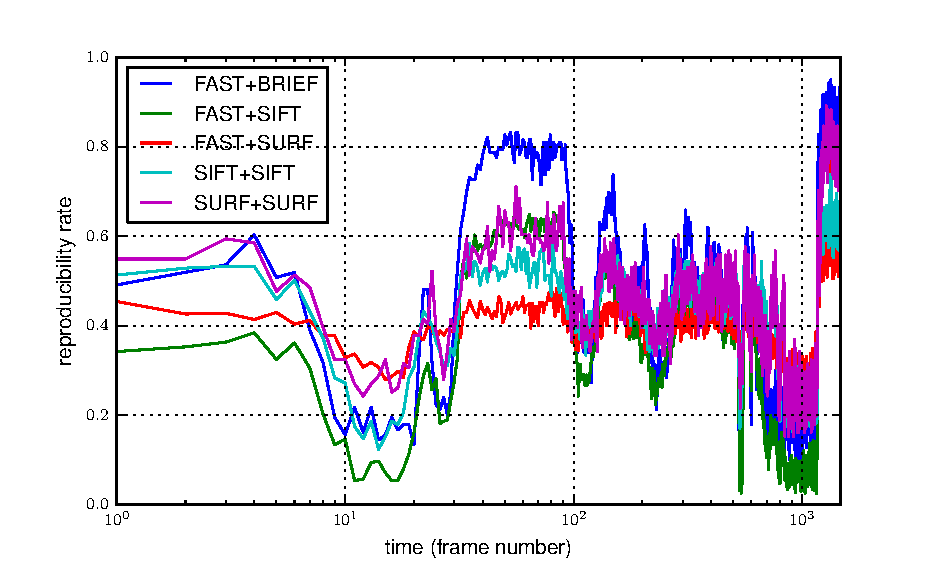
\includegraphics{../figures/reproducibility.pdf}
\end{figure}


\bibliography{bibliography}

%----------------------------------------------------------------------------------------

\end{document}